% !TEX encoding = UTF-8 Unicode
% !TEX TS-program = pdflatex
% !TEX root = ../Tesi.tex


%************************************************
\myChapter*{Introduzione}
%************************************************
\section{L'ottica adattiva nell'osservazione astronomica}
Negli ultimi decenni l'ottica adattiva si è ampiamente diffusa nell'ambito dell'osservazione astronomica come risposta alla necessità di aumento del potere risolutivo dei telescopi di grandi dimensioni: infatti è noto che, mentre in linea teorica la risoluzione (il più piccolo angolo di separazione in cui è possibile la distinzione di due oggetti osservati) è proporzionale alla dimensione della lente, nella realtà l'osservazione è soggetta a disturbi di diversa natura. Alcuni disturbi sono dovuti a tolleranze di costruzione, assemblaggio e installazione, mentre altri dipendono dalle condizioni operative dei telescopi stessi: deformazioni termiche, orientazione rispetto alla gravità, turbolenza atmosferica. Inoltre la sensibilità del potere risolutivo dei telescopi rispetto a questi disturbi, già molto elevata,  è proporzionale alla dimensione dei loro specchi. 

\begin{figure}[htb]
\centering
\caption{GMT design concept (\textcopyright\url{www.gmto.org})}
\label{fig:GMT}

\includegraphics[width = .9\textwidth]{GMT}
\end{figure}

Per questi motivi l'attenuazione dei disturbi tramite sistemi di controllo attivo è oggi la tecnologia di riferimento per l'osservazione astronomica terrestre, e gli studi per l'applicazione spaziale sono in rapida diffusione.\\

Per quanto riguarda le applicazioni terrestri, in cui la principale fonte di disturbo è la diffrazione causata dalla turbolenza atmosferica, lo stato dell'arte è rappresentato, in particolar modo, dai due modelli in fase di sviluppo qui riportati:
\begin{description}
 \item[GMT] -- \textit{Giant Magellan Telescope}
 \item[E-ELT] -- \textit{European Extremely Large Telescope}
\end{description}

Il primo, frutto della collaborazione di diversi enti e università e finanziato principalmente da Australia, USA e Korea, vanterà un parco di 7 specchi primari di diametro di 8.4 m con un potere risolutivo equivalente a quello di un singolo specchio di 24 m.
L'ottica adattiva sarà installata sullo specchio secondario (M2) di 3.1 m.
Il telescopio sarà operativo presso l'osservatorio di Las Campanas (Cile) nel 2018.\\



Il secondo, nato da un progetto ESO (\textit{European Southern Observatory}), sarà situato a Cerro Amazones (Cile) e vanterà un diametro dello specchio primario (M1) di 39 m e un sistema complessivo di 5 specchi, di cui uno attivo (M4) di diametro pari a 2.6 m. 
L'anno di realizzazione previsto è il 2024.

\begin{figure}[htb]
\centering
\caption{E-ELT design concept (\textcopyright\url{www.eso.org})}
\label{fig:EELT}
\includegraphics[width = .9\textwidth]{EELT}
\end{figure}




L'ottica adattiva compensa le aberrazioni del fronte d'onda in ingresso attraverso il controllo della deformazione di uno o più componenti ottici (specchi) del telescopio. 
In figura \ref{fig:control_global} è riportata la struttura di un sistema ottico attivo \citep{manetti_high_2010}:
\begin{itemize}
\item Attraverso un sistema di guide laser viene misurata la distorsione del fronte d'onda;
\item  Sulla base dell'elaborazione dell'aberrazione, un controllore ottico calcola la forma di riferimento che dovrà assumere l'elemento deformabile (adattivo);
\item La deformazione desiderata viene inviata al sistema di controllo strutturale dello specchio;
\item Attraverso un elevato numero di attuatori e sensori il controllore impone allo specchio l'inseguimento della forma desiderata, in modo tale da compensare l'aberrazione del fronte d'onda e garantire la cancellazione dei diversi rumori.
\end{itemize}
\begin{figure}[htb]
\centering
\caption{Struttura del sistema di controllo complessivo}
\label{fig:control_global}
\resizebox{\textwidth}{!}{%
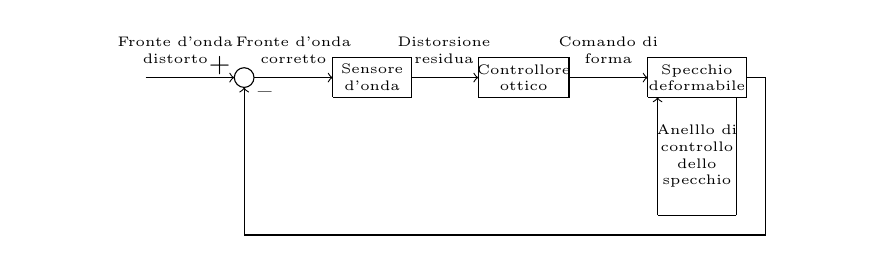
\begin{tikzpicture}[scale = .5]
    \draw[->] {(-4.75,.5) -- (-2.5,.5)};
    \draw  (-2.25,.5) circle (.25);
    \draw[->] {(-2,.5) -- (0,.5)};
    \draw (0,0) -- (2,0) -- (2,1) -- (0,1) -- (0,0);
    \draw[->] {(2,.5) -- (3.7,.5)};
    \draw (3.7,0) -- (6,0) -- (6,1) -- (3.7,1) -- (3.7,0);
    \draw[->] {(6,.5) -- (8,.5)};
    \draw (8,0) -- (10.5,0) -- (10.5,1) -- (8,1) -- (8,0);
    \draw {(10.5,.5) -- (11,.5)};
    \draw {(11,.5) -- (11,-3.5)};
    \draw {(11,-3.5) -- (-2.25,-3.5)};
    \draw[->] {(-2.25,-3.5) -- (-2.25,.25)};
    \draw {(10.25,0) -- (10.25,-3)};
    \draw {(10.25,-3) -- (8.25,-3)};
    \draw[->] {(8.25,-3) -- (8.25,0)};
    \draw (-2.35,.8) node[left] {+}; %label
    \draw (-2.15,.1) node[right] {--}; %label
    \tikzset{block/.append style={align = center , text width=10em,font=\tiny}}
    \draw (-4,1.2) node[block] {Fronte d'onda\\ distorto};
    \draw (1,0.5) node[block] {Sensore\\ d'onda};
    \draw (4.85,0.5) node[block] {Controllore\\ ottico};
    \draw (9.25,0.5) node[block] {Specchio\\ deformabile};
    \draw (9.25,-1.5) node[block] {Anelllo di \\ controllo\\ dello\\ specchio};
    \draw (-1,1.2) node[block] {Fronte d'onda\\ corretto};
    \draw (2.825,1.2) node[block] {Distorsione\\ residua};
    \draw (7,1.2) node[block] {Comando di\\ forma};
\end{tikzpicture}}
\end{figure}
\section{Elementi del sistema}

Lo specchio, che costituisce l'elemento strutturale deformabile, è una piastra sottile sospesa al di sopra di un corpo di riferimento rigido (\textit{reference body}). L'unico collegamento fra i due elementi è il sostegno centrale dello specchio il cui scopo è fornire un'elevata rigidezza nel piano e una modica rigidezza legata a movimenti trasversali. La distanza fra lo specchio sospeso e il riferimento è dell'ordine di $10^{-4}$ m. 

\begin{SCfigure}[2][htb]
\centering
\caption{Specchio deformabile di uno dei quattro telescopi che compongono il \textit{Very Large Telescope}, realizzato da ESO e situato a Cerro Paranal (\textcopyright\url{www.eso.org})}
\label{fig:shellVLT}

\includegraphics[width = .5\textwidth]{shellVLT}
\end{SCfigure}

Il reference body e lo specchio ospitano un gran numero di attuatori lineari a induzione collegati al sistema di controllo. Ciascun attuatore è circondato da un sensore capacitivo a corona circolare che permette la misura locale della distanza fra i due corpi. 

Il principio di attuazione è la forza magnetica scambiata fra un induttore solidale al reference body e un magnete permanente solidale alla piastra. 


Il sistema dinamico è formato da:
\begin{itemize}
\item Piastra deformabile
\item Reference body
\item Attuatori
\item Sensori
\end{itemize}

Sia per l'attuazione che per l'acquisizione le caratteristiche degli strumenti devono essere ben caratterizzate in funzione delle condizioni in cui operano. Particolare attenzione viene posta alla variazione del loro comportamento meccanico (in termini di forze e coppie) ed elettro-magnetico (induttanze, capacità e flussi concatenati) in funzione di posizione e rotazione relative degli elementi. 

Queste, a loro volta, dipendono da diversi fattori fra i quali: forma locale assunta dallo specchio, tolleranze di assemblaggio, disallineamenti dovuti a gravità e gradienti termici.

Lo scopo di questa tesi è l'analisi tramite simulazioni numeriche del comportamento degli attuatori e dei sensori adottati per il controllo dello specchio in funzione delle condizioni sopra citate e dell'impatto di questi ultimi nella simulazione del sistema controllato dello specchio di un telescopio. 

\begin{figure}[htb]
\centering
\caption{Reference body del Very Large Telescope (\textcopyright\url{www.eso.org})}
\label{fig:refVLT}

\includegraphics[width = .9\textwidth]{refVLT}
\end{figure}
\section{Strumenti utilizzati}
\'E stata fatta la scelta di effettuare tutte le simulazioni con il linguaggio di programmazione \textit{Python}, utilizzando le librerie dedicate al calcolo numerico \textit{numpy} \citep{numpy}, l'insieme di \textit{tool} grafici \textit{matplotlib} \citep{Hunter:2007} e soprattutto l'ambiente \textit{FEniCS} \citep{LoggMardalEtAl2012a} - in particolare il pacchetto \textit{Dolfin} \citep{LoggWellsEtAl2012a} - versatile insieme di librerie dedicate alla risoluzione di equazioni differenziali mediante il metodo agli elementi finiti. Punto di forza di FEniCS è la possibilità di risolvere problemi differenziali complessi sulla base dell'espressione del problema in forma debole e della griglia di calcolo (\textit{mesh}). \\

Il pacchetto permette di eseguire agevolmente le operazioni di assemblaggio delle matrici e di estrapolazione dei risultati. Per questo è stato scelto come strumento principale sia per le analisi elettromagnetiche (grazie anche alla possibilità di utilizzare la classe di elementi di Nèdèlèc) sia per le analisi strutturali (così da integrare direttamente il controllore in forma digitale rimanendo nello stesso ambiente di sviluppo). 

Per la generazione delle griglie di calcolo è stato utilizzato il programma \textit{Gmsh} \citep{gmsh}. 

Infine, le operazioni di \textit{post-processing} - laddove non sono state effettuate tramite Fenics - hanno richiesto l'utilizzo del programma \textit{Paraview} \citep{paraview}.\\ 

Tutti gli strumenti utilizzati sono open-source.\\

\begin{center}
\begin{tabular}{c}
\toprule
     
\includegraphics[width = .5\textwidth]{python-banner}\\
     
\includegraphics[width = .5\textwidth]{numpy-banner}\\
     
\includegraphics[width = .5\textwidth]{matplotlib-banner}\\
     
\includegraphics[width = .5\textwidth, height = .1\textwidth]{fenics-banner}\\
     
\includegraphics[width = .5\textwidth]{gmsh-banner}\\
     
\includegraphics[width = .5\textwidth]{paraview-banner}\\
\bottomrule
\end{tabular}
\end{center}
\section{Organizzazione del lavoro}


\begin{description}
\item[Nella prima parte] sono illustrati e validati i modelli matematici utilizzati per le analisi elettromagnetiche. In particolare:
  \begin{description}
  \item[Nel Capitolo \ref{cap:maxwell}] dopo aver richiamato brevemente le equazioni di Maxwell, vengono analizzati i modelli costitutivi, i regimi ridotti e gli schemi a potenziale.
  \item[Nel Capitolo \ref{cap:boundary}] sono elencate le condizioni al contorno e di interfaccia implementate. Viene inoltre mostrato lo sviluppo di una tecnica di trasformazione al contorno per l'analisi in domini aperti. Infine si verifica l'applicabilità delle ipotesi adottate per le condizioni al contorno nelle regioni metalliche. 
  \item[Nel Capitolo \ref{cap:bvp}] è illustrata la costruzione della forma variazionale del problema elettromagnetico e la conseguente scelta delle classi di elementi finiti adatte alla simulazione numerica.
  \item[Nel Capitolo \ref{cap:output}] viene posta attenzione al calcolo di forze e coppie, induttanze, flussi concatenati e capacità.
  \end{description}
\item[Nella seconda parte] si utilizzano i modelli sviluppati per l'analisi di un gruppo sensore-attuatore in fase di sviluppo. Viene inoltre generato un modello strutturale dello specchio per una valutazione del loro impatto sulle prestazioni del sistema di controllo. Più in dettaglio:
  \begin{description}
  \item[Nel Capitolo \ref{chap:ActSens}] vengono mostrati i risultati ottenuti per il gruppo di controllo preso in esame, analizzando forze e coppie scambiate, induttanze, flussi concatenati e capacità. 
  \item[Nel Capitolo \ref{chap:mirror}] vengono brevemente introdotti lo sviluppo del modello strutturale di uno specchio, la struttura del sistema di controllo e l'algoritmo di integrazione diretta nel tempo.
  \item[Nel Capitolo \ref{chap:simulations}] è analizzato l'effetto della modellazione di attuatori e sensori sulla simulazione diretta nel tempo della dinamica dello specchio durante l'inseguimento di una storia della durata di un secondo. Vengono proposte soluzioni per una migliore ricostruzione della velocità dei punti di controllo per un aumento della robustezza del sistema. Infine, viene impostato il controllo in tensione con controreazione proporzionale in corrente come alternativa al controllo in corrente.
  \item[Il Capitolo \ref{chap:Conclusioni}] riassume brevemente le conclusioni del lavoro e gli sviluppi futuri.
  \end{description}
\end{description}



